%% The following is a directive for TeXShop to indicate the main file
%%!TEX root = diss.tex

\chapter{Interpretation of 3D Reconstruction Model}
\label{ch:3DRecon_Interp}
In order to validate the 3D reconstruction taxonomy and the model derived from it, interpretability from the object centric model into appropriate solutions must be shown. Our interpreter is based on the direct evaluation of the performance of each 3D reconstruction algorithm under different conditions presented in Chapter~\ref{ch:3DRecon_Benchmark}. From this analysis of how algorithms perform on objects which have different visual and geometric properties, an algorithm(s) can be definitively chosen based on which performed best on the training images.

The three algorithms introduced in our test bench are: the PMVS proposed by \citeauthor{furukawa2010accurate}, the example-based Photometric Stereo proposed by \citeauthor{hertzmann2005example}, and a standard gray-coded Structured Light technique with error rejection.

Although there are only three algorithms selected, all of them are the top performers in the corresponding field, and are sufficient to demonstrate the framework's ability to translate the descriptive model into a reconstruction. The integration of a new algorithm requires only that they be evaluated with a similar procedure and images presented in Chapter~\ref{ch:3DRecon_Benchmark}, allowing researchers to contribute novel algorithms to the framework. The source code and blender files used to generate the images are available online to encourage the testing of additional algorithm, and incorporation of additional properties.

\section{Synthetic Datasets}


\section{Real-world Datasets}
We use the dataset `cup' as an example. The property of the `cup' is listed in Table~\ref{tab:prop_list_cup}.

\begin{table}[h]
  \centering
  \begin{tabular}{l*{4}{c}}
  \hline
  \textbf{Property} & Texture coverage & Albedo & Specularity & Roughness\\
  \hline
  cup & 0.2 & 0.8 & 0.8 & 0.2\\
  \hline
  \end{tabular}
  \label{tab:prop_list_cup}
  \caption{Property list for the real-world objects}
\end{table}

From the trained performance of each technique as shown in Figure~\ref{fig:train_cup}
\begin{figure}[h!]
\begin{tabular}{ccc}
\includegraphics[width=0.33\textwidth]{interp/mvs_train}&
\includegraphics[width=0.33\textwidth]{interp/ps_train}&
\includegraphics[width=0.33\textwidth]{interp/sl_train}\\
(MVS) & (PS) & (SL)\\
\end{tabular}
\caption{Performance of MVS, PS, and SL with varied properties}
\label{fig:train_cup}
\end{figure}

From the trained performance, we can clearly see that MVS performs poorly, as it ranks fifth among all 9 combinations, after 020802, 020502, 020805, 020505 (order of property as previously stated), thus we conclude that MVS is not suitable for	`cup'.

From the performance of PS, we can see that it performs well in this case, as the mean and median angle different is below $10^\circ$, and mean and median are not far apart, suggesting that there is no spikes.

From the performance of SL, we can see that it ranks top 3 among all 9 combinations in terms of completeness, thus SL also does a decent job reconstructing `cup'.

Following the same methods, we obtain the best-suited algorithm(s) for all the other objects as shown in Table~\ref{tab:prop_list_real_world_obj}.

\begin{table}[h]
  \centering
  \begin{tabular}{l*{5}{c}}
  \hline
  \textbf{Property} & Texture coverage & Albedo & Specularity & Roughness & Best-suited Algo.\\
  \hline
  box & 0.8 & 0.8 & 0.2 & 0.2 & MVS, SL, PS\\
  cat0 & 0.5 & 0.2 & 0.5 & 0.2 & None\\
  cat1 & 0.2 & 0.2 & 0.8 & 0.2 & None\\
  cup & 0.2 & 0.8 & 0.8 & 0.2 & PS, SL\\
  dino & 0.2 & 0.5 & 0.2 & 0.5 & PS, SL\\
  house & 0.8 & 0.2,0.8 & 0.8 & 0.2 & MVS\\
  pot & 0.5 & 0.2,0.5 & 0.2 & 0.2 & MVS, SL\\
  status & 0.2 & 0.8 & 0.5 & 0.2 & PS, SL\\
  vase & 0.8 & 0.2 & 0.8 & 0.2 & MVS\\
  \hline
  \end{tabular}
  \label{tab:prop_list_real_world_obj}
  \caption{Property list for the real-world objects}
\end{table}

Here we show the reconstruction of the real-world datasets. Since we don't have the ground truth, visual 

\begin{figure}[h!]
\centering
\begin{tabular}{lcccr}
Object & MVS & PS & SL & Best-suited Algo.\\
box &
\raisebox{-.5\height}{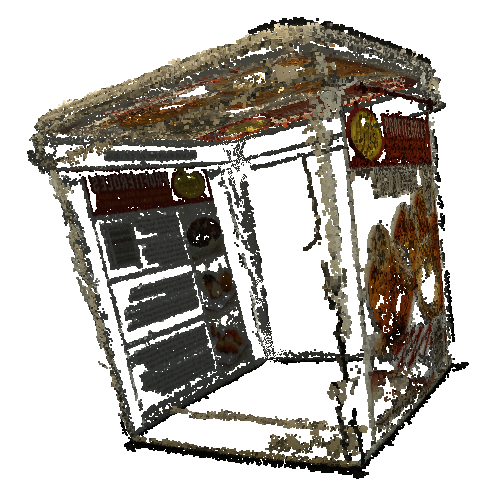
\includegraphics[width=0.2\textwidth]{interp/box_mvs_00}}&
\raisebox{-.5\height}{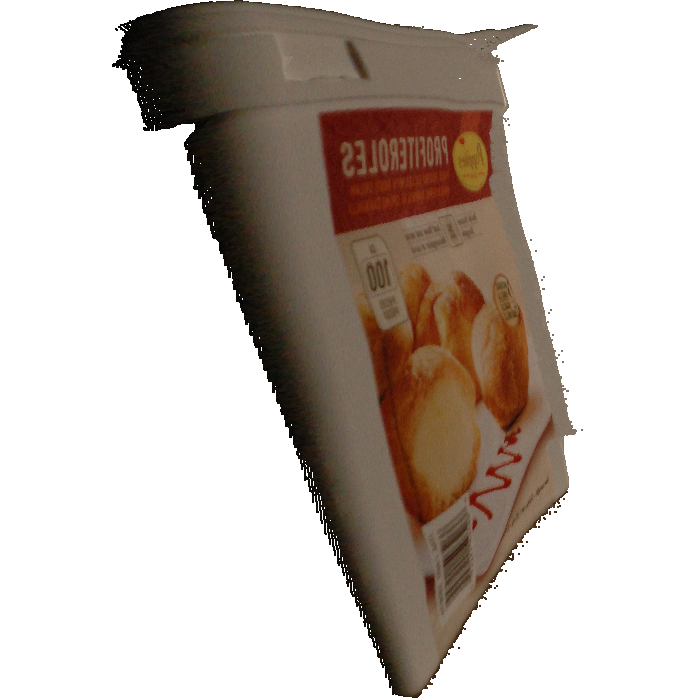
\includegraphics[width=0.2\textwidth]{interp/box_ps_00}}&
\raisebox{-.5\height}{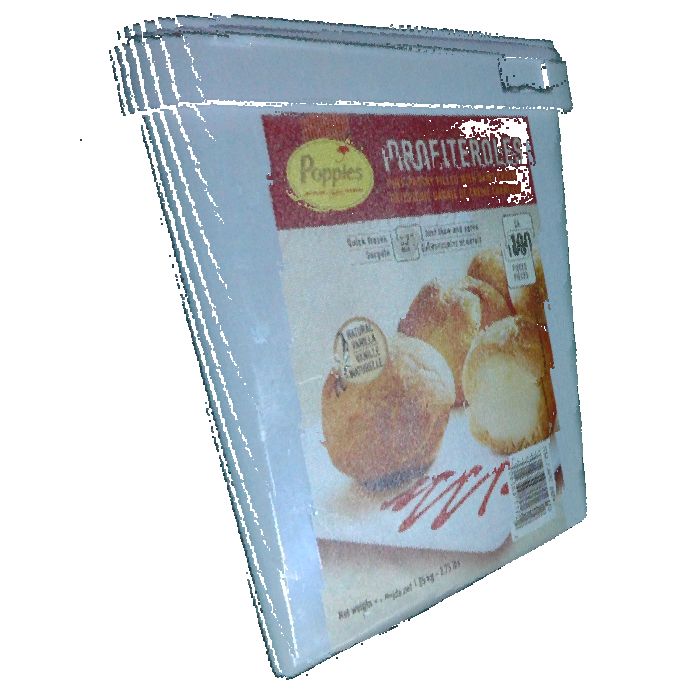
\includegraphics[width=0.2\textwidth]{interp/box_sl_00}}&
MVS, SL, PS\\
cat0 &
\raisebox{-.5\height}{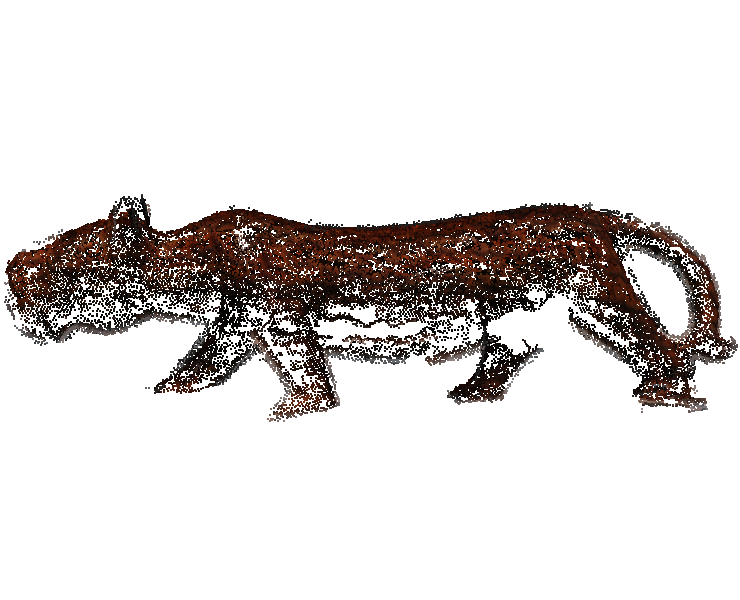
\includegraphics[width=0.2\textwidth]{interp/cat0_mvs_00}}&
\raisebox{-.5\height}{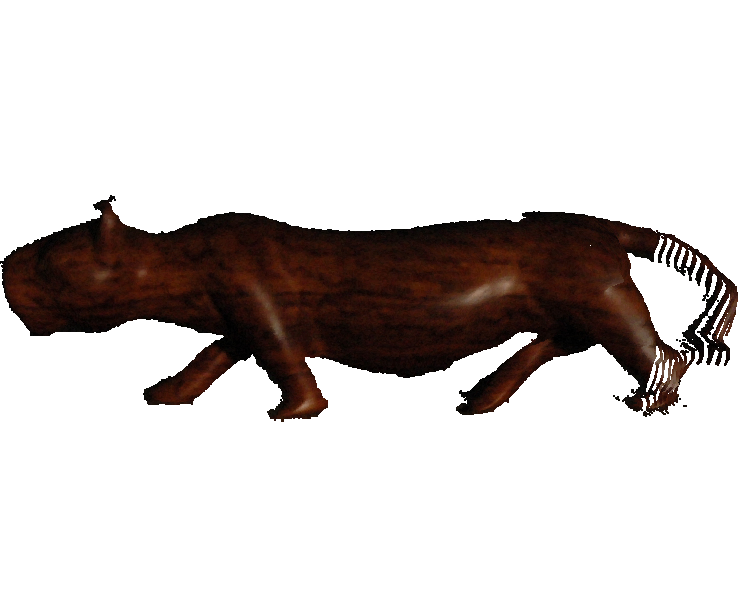
\includegraphics[width=0.2\textwidth]{interp/cat0_ps_00}}&
\raisebox{-.5\height}{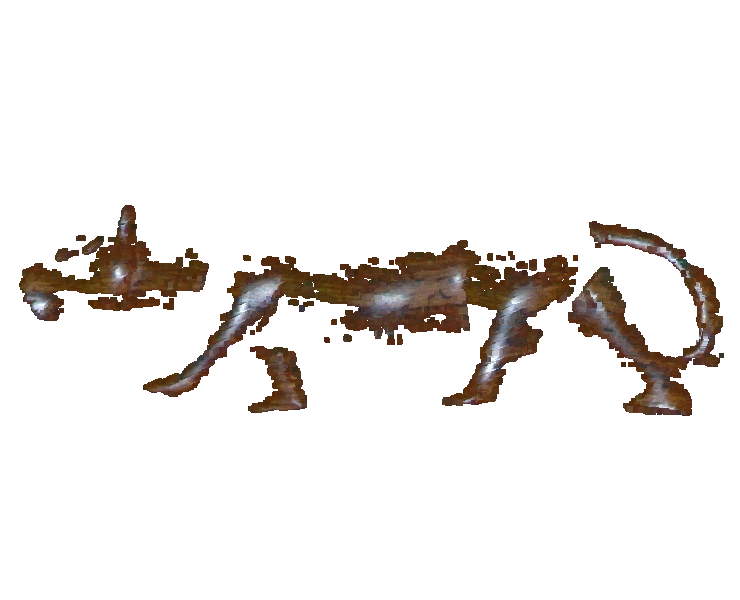
\includegraphics[width=0.2\textwidth]{interp/cat0_sl_00}}&
None\\
cat1 &
\raisebox{-.5\height}{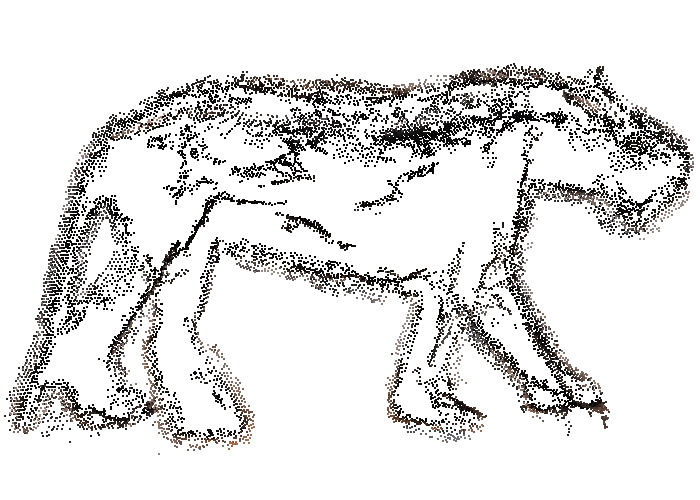
\includegraphics[width=0.2\textwidth]{interp/cat1_mvs_00}}&
\raisebox{-.5\height}{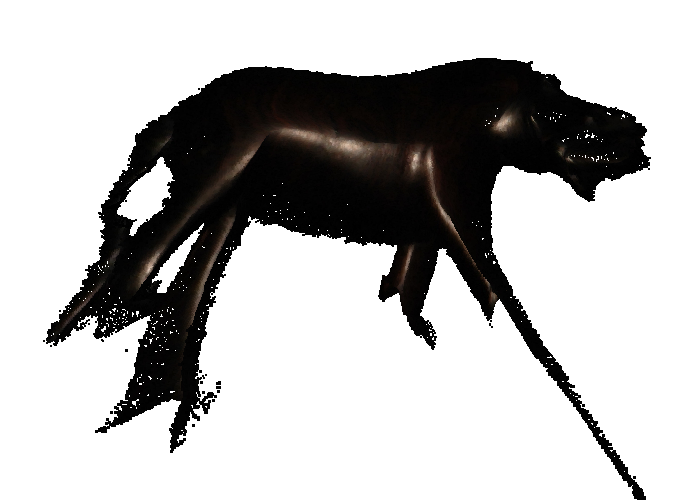
\includegraphics[width=0.2\textwidth]{interp/cat1_ps_00}}&
\raisebox{-.5\height}{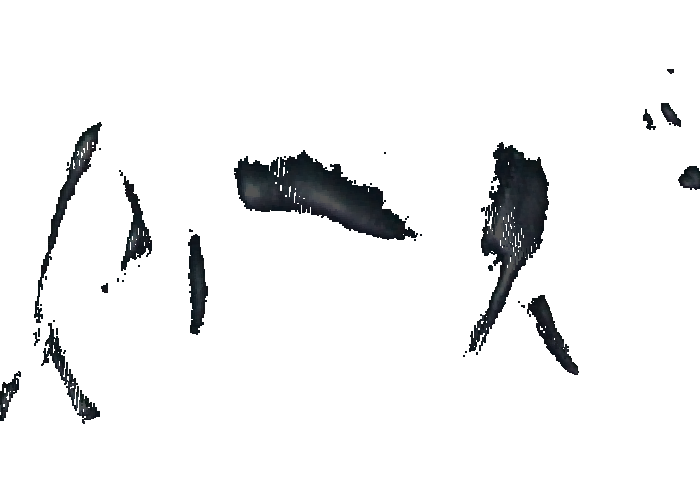
\includegraphics[width=0.2\textwidth]{interp/cat1_sl_00}}&
None\\
dino &
\raisebox{-.5\height}{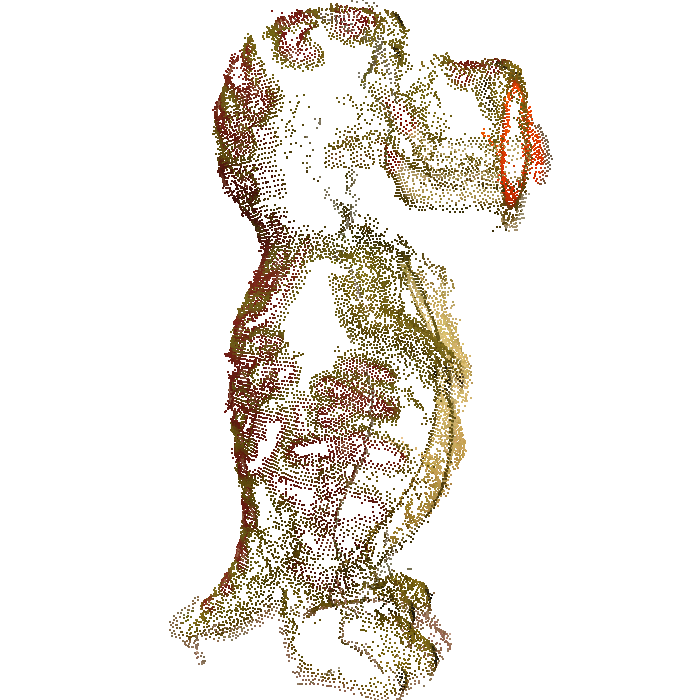
\includegraphics[width=0.2\textwidth]{interp/dino_mvs_00}}&
\raisebox{-.5\height}{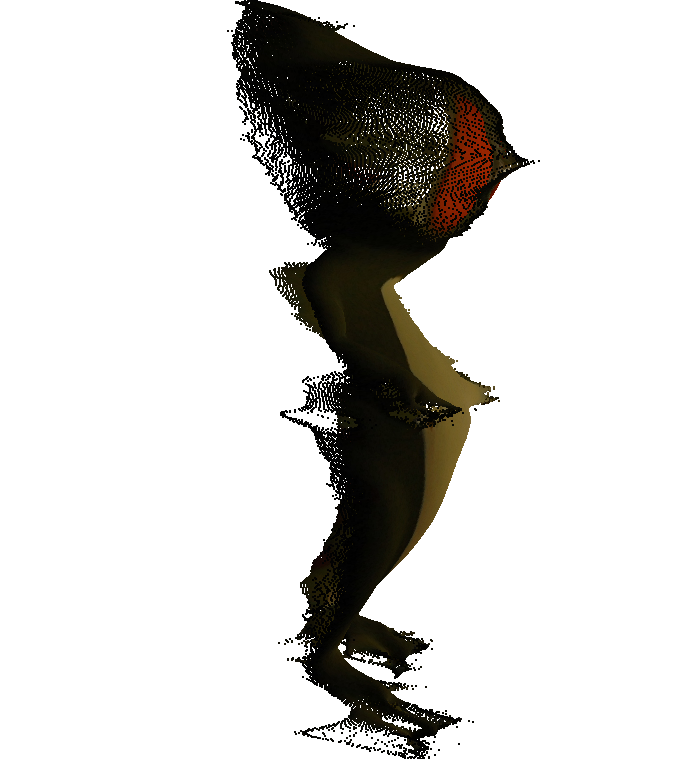
\includegraphics[width=0.2\textwidth]{interp/dino_ps_00}}&
\raisebox{-.5\height}{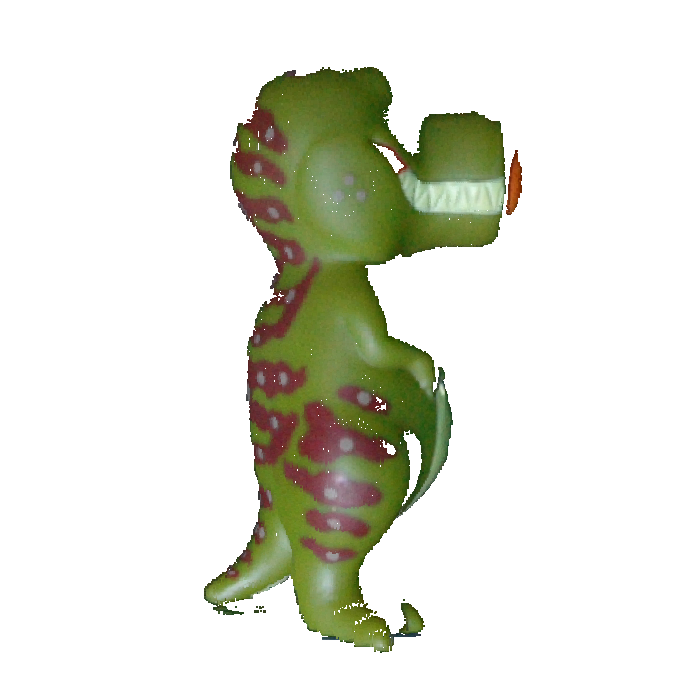
\includegraphics[width=0.2\textwidth]{interp/dino_sl_00}}&
PS, SL\\
cup &
\raisebox{-.5\height}{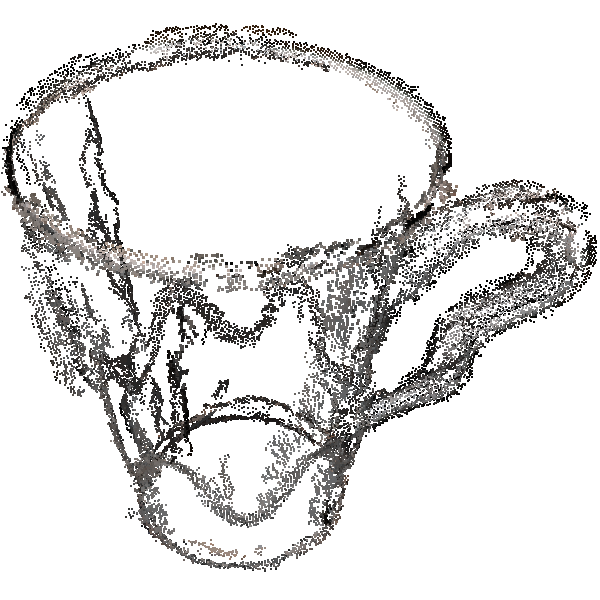
\includegraphics[width=0.2\textwidth]{interp/cup_mvs_00}}&
\raisebox{-.5\height}{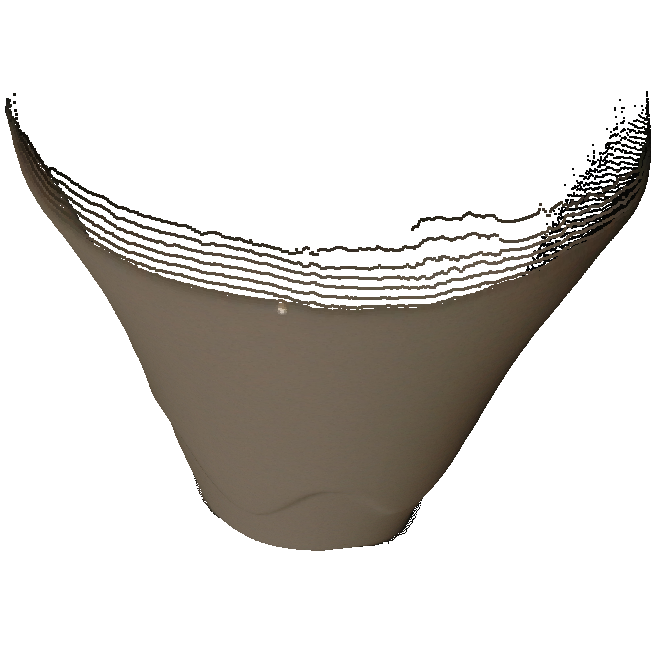
\includegraphics[width=0.2\textwidth]{interp/cup_ps_00}}&
\raisebox{-.5\height}{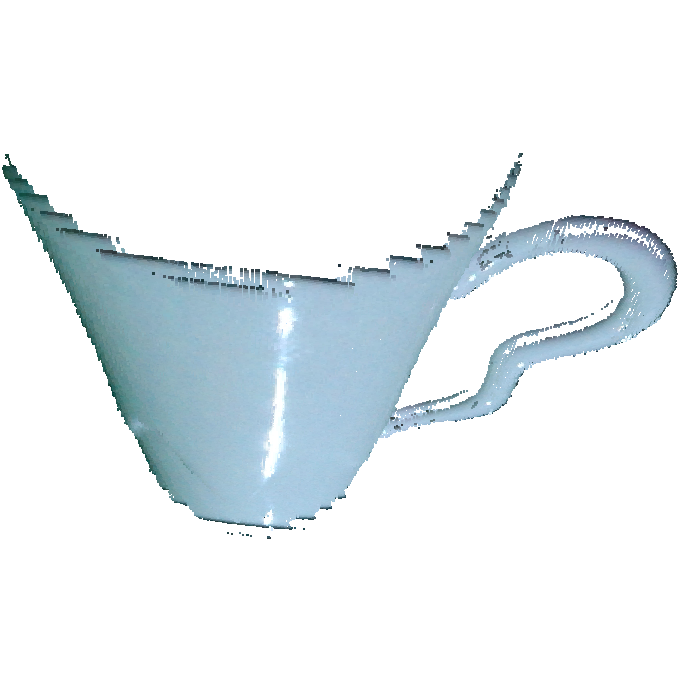
\includegraphics[width=0.2\textwidth]{interp/cup_sl_00}}&
PS, SL\\
house &
\raisebox{-.5\height}{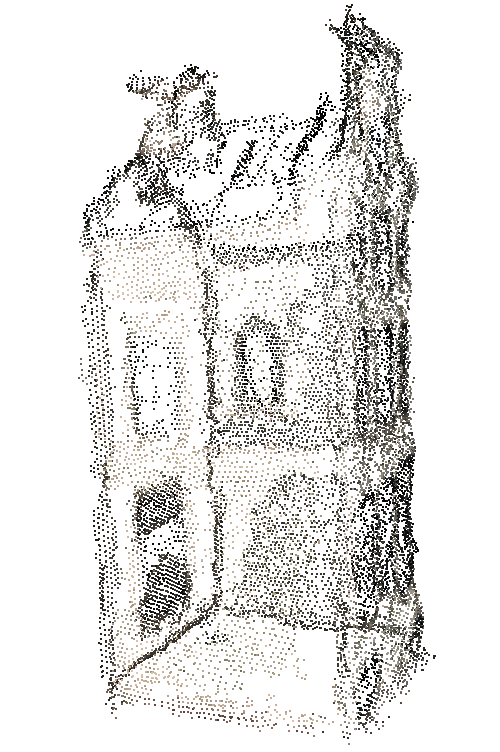
\includegraphics[width=0.2\textwidth]{interp/house_mvs_00}}&
\raisebox{-.5\height}{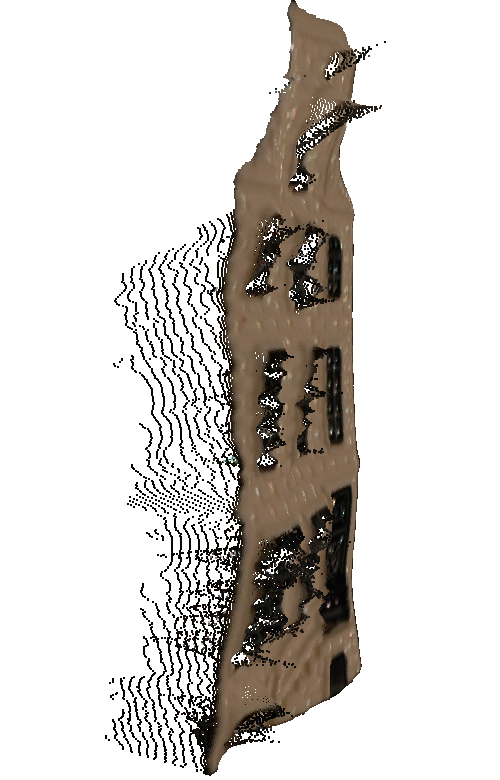
\includegraphics[width=0.2\textwidth]{interp/house_ps_00}}&
\raisebox{-.5\height}{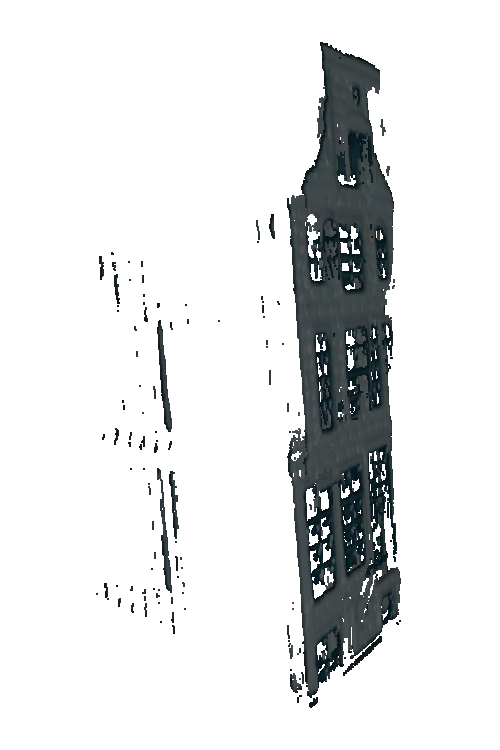
\includegraphics[width=0.2\textwidth]{interp/house_sl_00}}&
MVS\\
pot &
\raisebox{-.5\height}{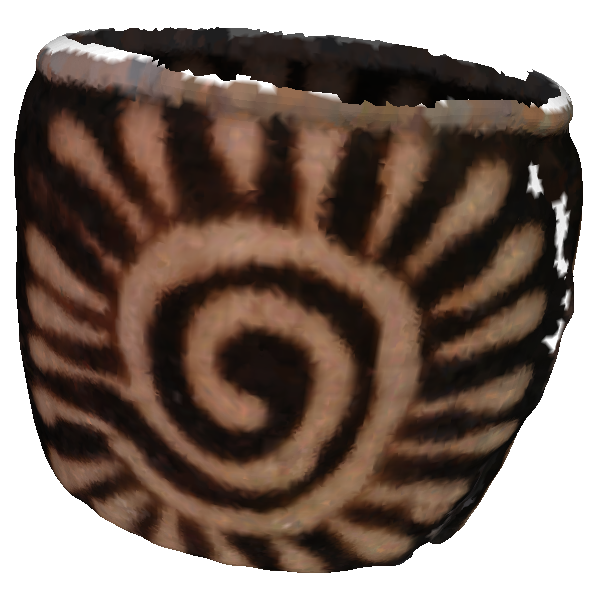
\includegraphics[width=0.2\textwidth]{interp/pot_mvs_01}}&
\raisebox{-.5\height}{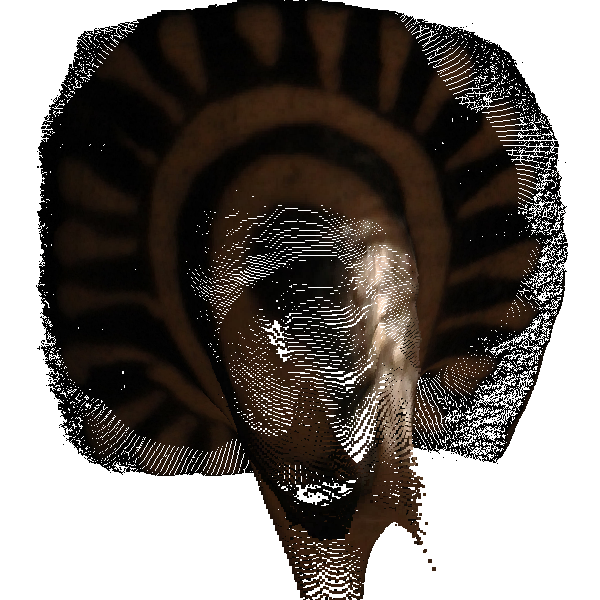
\includegraphics[width=0.2\textwidth]{interp/pot_ps_00}}&
\raisebox{-.5\height}{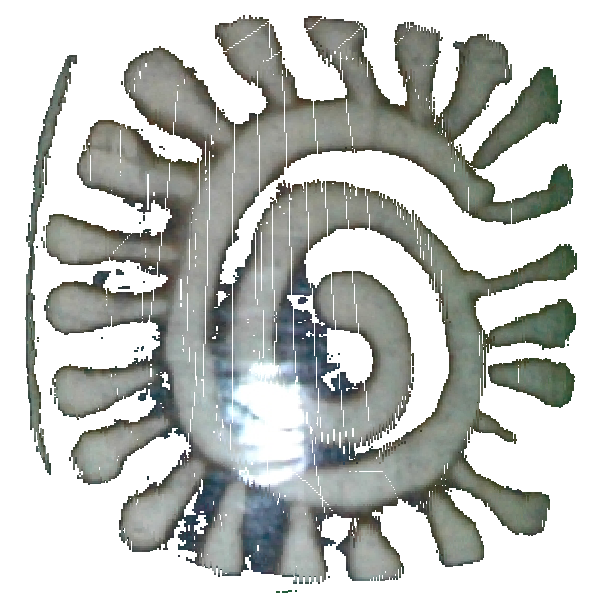
\includegraphics[width=0.2\textwidth]{interp/pot_sl_00}}&
MVS, SL\\
\end{tabular}
\caption{Reconstruction results of MVS, PS, SL}
\label{fig:test_real_world_obj}
\end{figure}

\begin{figure}[h!]
\centering
\begin{tabular}{lcccr}
Object & MVS & PS & SL & Best-suited Algo.\\
statue &
\raisebox{-.5\height}{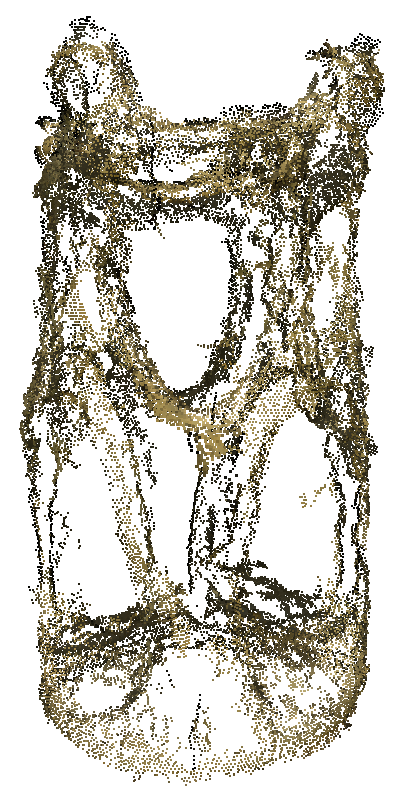
\includegraphics[width=0.2\textwidth]{interp/statue_mvs_00}}&
\raisebox{-.5\height}{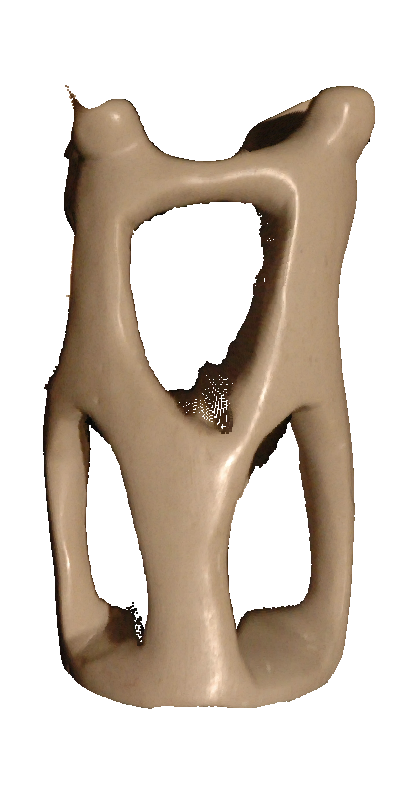
\includegraphics[width=0.2\textwidth]{interp/statue_ps_00}}&
\raisebox{-.5\height}{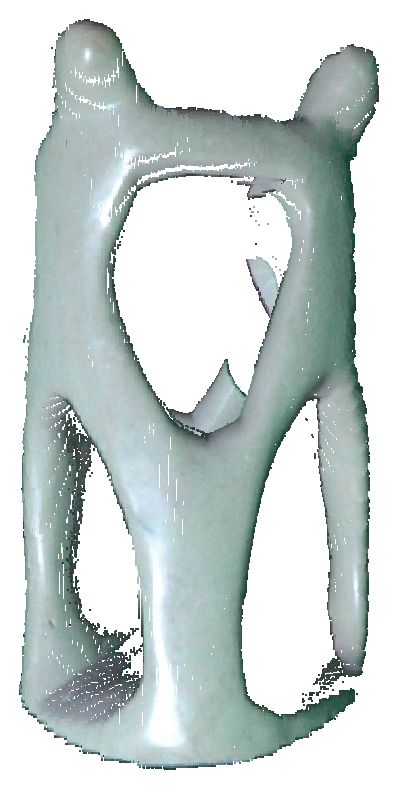
\includegraphics[width=0.2\textwidth]{interp/statue_sl_00}}&
PS, SL\\
vase &
\raisebox{-.5\height}{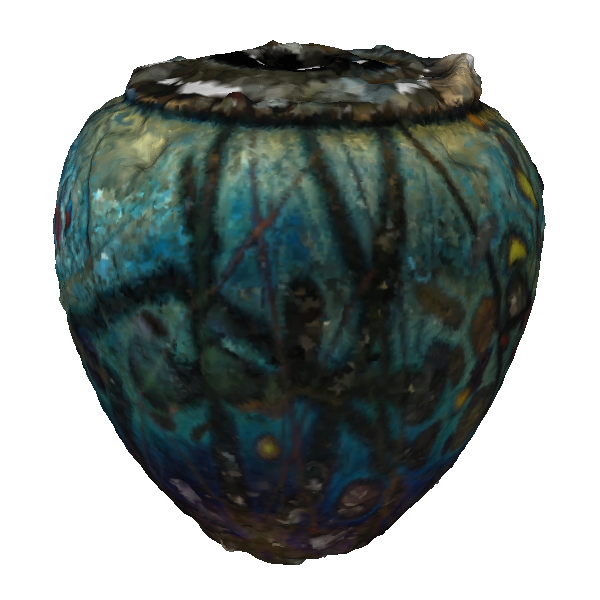
\includegraphics[width=0.2\textwidth]{interp/vase_mvs_01}}&
\raisebox{-.5\height}{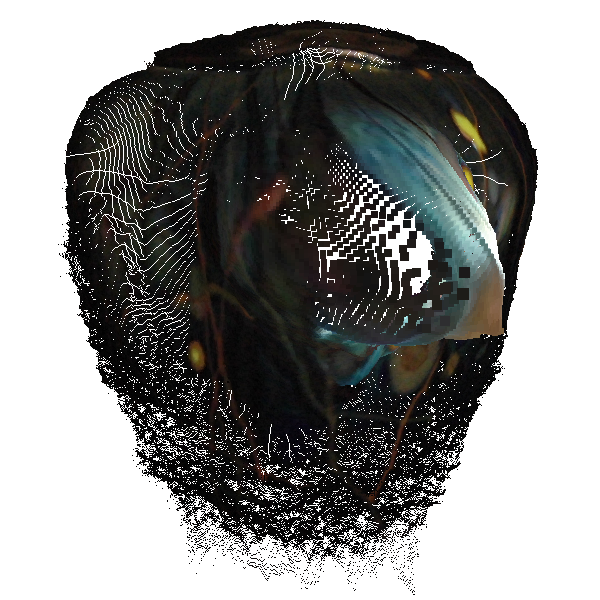
\includegraphics[width=0.2\textwidth]{interp/vase_ps_00}}&
\raisebox{-.5\height}{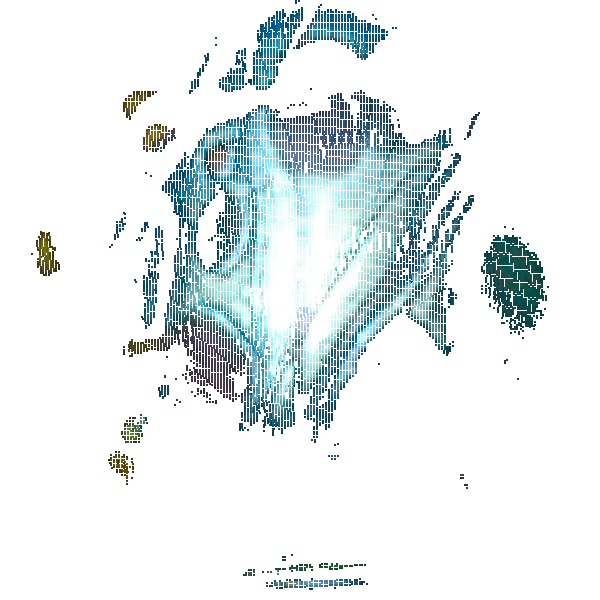
\includegraphics[width=0.2\textwidth]{interp/vase_sl_00}}&
MVS\\
\end{tabular}
\caption{Reconstruction results of MVS, PS, SL (cont'd)}
\label{fig:test_real_world_obj}
\end{figure}

\section{Observations}
\begin{itemize}
\item roughness on ps
\item low albedo, high specularity on SL
\item low albedo, high specularity, low roughness, high spikes
\end{itemize}

\section{Summary}

